\documentclass{beamer}

% do the following to "grey out" previous bulleted items
% and couple with:
%   \begin{itemize}[<+>]
\setbeamercovered{invisible}
\setbeamercovered{%
  again covered={\opaqueness<1->{35}}}


%\usepackage{beamerthemesplit}
%\usetheme{Madrid}
\usetheme{Warsaw} % my favourite
%\usetheme{Malmoe}
%\usetheme{Szeged} % this one is a bit different


% this example will not work with natbib package
% if you are building locally, ensure 
% your Makefile is calling biber, not biblatex
\usepackage[
  style=apa,
  citestyle=authoryear,
  natbib=true,
  backend=biber
  ]{biblatex}
\bibliography{../documentRef}

% maths notation
\usepackage{amsmath}
% for labelling matrices
\usepackage{template/kbordermatrix}
\usepackage{mathtools}
% shorthand for matrix notation
% e.g. instead of boldface letter
\newcommand\mat[1]{\mathcal{#1}}


% make the references small text
\renewcommand*{\bibfont}{\normalfont\tiny}



\title{My Example Presentation}
\author{Boaty McBoatface}
\institute{ResBaz 2022}
\date{\today}


\begin{document}

\begin{frame}
\titlepage % beamer's \maketitle
\end{frame}


\frame{\tableofcontents}

%%%%%%%%%%%%%%%%%%%%%%%%%%%%%%%%%%%%%%%%%%%%%%%%%%%%%%%%%%%%%%%%%%%%%%%%%%%%%%%
%%% Introduction
%%%%%%%%%%%%%%%%%%%%%%%%%%%%%%%%%%%%%%%%%%%%%%%%%%%%%%%%%%%%%%%%%%%%%%%%%%%%%%%


\section{Section 1}
\begin{frame}
    \Huge{The first section}
\end{frame}

\subsection{A simple frame}
\begin{frame}
    Some text
    \begin{itemize}
        \item a bullet 
        \item another bullet
    \end{itemize}
\end{frame}


\subsection{A simple frame with greyed out bullets}
\begin{frame}
    Some text
    \begin{itemize}[<+>]
        \item a bullet 
        \item another bullet
        \item the very last bullet
    \end{itemize}
\end{frame}


\section{Section 2}
\begin{frame}
    \Huge{The second section}
\end{frame}

\subsection{Blocks}
\begin{frame}
    \begin{block}{a normal block}
        \begin{itemize}
            \item 1
            \item 2
            \item 3
        \end{itemize} 
    \end{block}
\end{frame}

\begin{frame}
    \begin{exampleblock}{an exampleblock}
        \begin{itemize}
            \item a
            \item b
            \item c
        \end{itemize} 
    \end{exampleblock}
\end{frame}

\begin{frame}
    \begin{alertblock}{an alertblock}
        \begin{itemize}
            \item x1
            \item x2
            \item x3
        \end{itemize} 
    \end{alertblock}
\end{frame}

\subsection{Columns}
\begin{frame}
    Frames can have columns
    \begin{columns}[T]
        \begin{column}{.5\textwidth}
            \begin{itemize}[<+>]
                \item bullet 1
                \item bullet 2
                \item bullet 3
            \end{itemize} 
        \end{column}
        \begin{column}{.5\textwidth}
            \begin{block}{}
                % Your image included here
                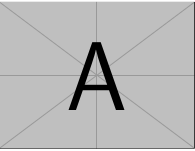
\includegraphics[width=\textwidth]{images/examples/image-a.png}
            \end{block}
        \end{column}
    \end{columns}
\end{frame}

\begin{frame}
    Blocks can be put in columns also
    \begin{columns}[T]
        \begin{column}{.5\textwidth}
            \begin{block}{}
                \begin{itemize}[<+>]
                    \item bullet 1
                    \item bullet 2
                    \item bullet 3
                \end{itemize} 
            \end{block}
        \end{column}
        \begin{column}{.5\textwidth}
            \begin{block}{}
                % Your image included here
                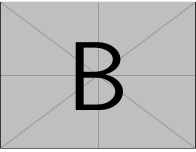
\includegraphics[width=\textwidth]{images/examples/image-b.png}
            \end{block}
        \end{column}
    \end{columns}
\end{frame}



% print the references if you like

% \begin{frame}[allowframebreaks]
%     \frametitle{References}
%     \printbibliography{}
% \end{frame}


\end{document}


